% Introduction to Programming · Nova SBE 2026/27 · Class 4 — Rules, judge, loop
%
%   ./build.sh            → build/class-4.pdf and build/class-4-notes.pdf
%
% Loops and transcripts are authored in Mermaid under diagrams/ and rendered to PDF by
% render-diagrams.py; this file only includes the results. The timelines and the git act are
% drawn in TikZ instead — see the theme: Mermaid could not hold them still or fill the width.
\documentclass[aspectratio=169,10pt]{beamer}
\usepackage{theme/beamerthemenovasbe}
% \tanote{} blocks are written once; the notes build shows them on a second screen.
% Without an explicit 'hide notes', beamer still lays each note out and overfills a box.
\ifdefined\WITHNOTES\setbeameroption{show notes on second screen=right}\fi

\setfootertext{Introduction to Programming · Class 4 · Nova SBE}
\title{Rules, judge, loop}
\subtitle{Agentic coding standards, part I}
\author{Nova SBE · Introduction to Programming 2026/27}
\date{22 September 2026}

\newcommand{\arr}{\,{\color{NovaMuted}$\rightarrow$}\,}

\begin{document}

% ═════════════════════════════════════════════ ACT 0 · open
\sectionslide[NovaTeal]{W4}{Block 1 · Class 4 · Practical}{Rules, judge, loop.}%
{Last week you watched a feature get built. Today you build one.}
\tanote{Timing: open + check-in 5 · what an agent is 17 · three standards 13 · git standards 5 ·
live kick-off 10 · your turn 30 · retro 6 · wrap 2 = 88, plus the two dividers. TA-run. Slides carry ideas
only: every command is on the Week 4 page, open on their laptops, and in these notes. Presenting
laptop: SplitIt with feature 1 merged, clean main, Codex open, GitHub Desktop signed in, data reset.}

% ── 2 · today
\hue{NovaTeal}
\begin{frame}{Today.}
\framesubtitle{Class 4}
\vspace*{\fill}
\begin{steps}
  \item Check-in
  \item What an agent actually is
  \item Three standards
  \item Git: one change, start to finish
  \item Build one, live — then you build one
  \item Retro: one new rule
\end{steps}
\vfill
\end{frame}

% ── 3 · check-in
\hue{NovaTeal}
\begin{frame}{Your GitHub page.}
\framesubtitle{Check-in · 5 min}
\vspace*{\fill}
\begin{itemize}
  \item A branch for feature 1.
  \item A merged pull request.
\end{itemize}
\vskip5mm
\muted{Not there yet? Start there today.}
\vfill
\end{frame}
\tanote{Walk the room looking at browsers, not code. Two minutes per row; note who is behind.
They can pull main and run the feature-1 tests while you walk; the command is on the Week 4 page.
Don't debug git at the front: point at last week's "when git is confusing" slide.}

% ═════════════════════════════════════════════ ACT 1 · what an agent is
\hue{NovaPurple}
\begin{frame}{Chat model, or agent.}
\framesubtitle{What is an agent?}
\vspace*{\fill}
\begin{tcbitemize}[cardsS, raster columns=2]
  \carditem{A chat model}{Text in, text out.}{It has never seen your folder.}
  \carditem{An agent}{The same model, with hands.}{Reads. Edits. Runs. Sees the result.
    Chooses again.}
\end{tcbitemize}
\vskip6mm
{\large\color{NovaFg}\textbf{Agent \;=\; model \;+\; tools \;+\; a loop.}}
\vfill
\end{frame}
\tanote{One minute, from their own experience: in Class 2 they asked Codex to show a line of a data
file and it showed the real line. A browser chat could not have. Same model family, different
powers. "Agentic" just means: can act, not only answer.}

% ── 5 · what a tool is
% The old version was two thin mermaid strips of boxes. The asymmetry that matters was in the
% card text and not in the picture: with tools, the result comes back to the MODEL. Here the
% return arrow carries it, and its length is the argument — short in the top lane (it comes back
% to you), full width in the bottom (it comes back to the thing doing the work).
\hue{NovaPurple}
\begin{frame}{Tools.}
\framesubtitle{What is an agent?}
\vspace*{\fill}
\noindent%
\begin{tikzpicture}[x=1mm, y=1mm]
  \useasboundingbox (0,-53) rectangle (134,4);
  % ── without tools: you are the hands, and you are the one who finds out
  \node[gp eyebrow=NovaMuted] at (0,1.2) {\lsp[13]{WITHOUT TOOLS}};
  \path[gp card=NovaCard] (0,-1) rectangle (134,-23);
  \icmodel[NovaMuted]{22}{-8.5}
  \icperson[NovaMuted]{67}{-8.5}
  \iclaptop[NovaMuted]{112}{-8.5}
  \node[gp body] at (22,-14) {the model};
  \node[gp body] at (67,-14) {you};
  \node[gp body] at (112,-14) {your laptop};
  \draw[gp move=NovaMuted] (29,-8.5) -- (60,-8.5);
  \node[gp movelabel=NovaBody, anchor=south] at (44.5,-7.7) {advice};
  \draw[gp move=NovaMuted] (75,-8.5) -- (104,-8.5);
  \node[gp movelabel=NovaBody, anchor=south] at (89.5,-7.7) {you type it};
  \draw[gp move=NovaMuted, rounded corners=1.4mm] (112,-17.5) -- (112,-19.8) -- (67,-19.8);
  \node[gp body, anchor=center, fill=NovaCard, inner xsep=1.8mm, inner ysep=0.5mm] at (89.5,-19.8) {you find out};
  % ── with tools: the same model, but the result lands back where the work happens
  \node[gp eyebrow=NovaBlue] at (0,-26.8) {\lsp[13]{WITH TOOLS}};
  \path[gp card=NovaBlueBg] (0,-29) rectangle (134,-51);
  \icmodel[NovaPurple]{22}{-36.5}
  \icgear[NovaBlue]{67}{-36.5}
  \iclaptop[NovaBlue]{112}{-36.5}
  \node[gp body] at (22,-42) {the model};
  \node[gp body] at (67,-42) {Codex};
  \node[gp body] at (112,-42) {your laptop};
  \draw[gp move=NovaBlue] (29,-36.5) -- (60,-36.5);
  \node[gp movelabel=NovaBlue, anchor=south] at (44.5,-35.7) {read · edit · run};
  \draw[gp move=NovaBlue] (74,-36.5) -- (104,-36.5);
  \node[gp movelabel=NovaBlue, anchor=south] at (89,-35.7) {does it};
  \draw[gp move=NovaBlue, rounded corners=1.4mm] (112,-45.5) -- (112,-47.8) -- (22,-47.8);
  \node[gp body, anchor=center, fill=NovaBlueBg, inner xsep=1.8mm, inner ysep=0.5mm] at (67,-47.8) {\textbf{it} finds out};
\end{tikzpicture}%
\vskip3mm
\muted{The same model both times. What changes is who finds out that it was wrong.}
\vfill
\end{frame}
\tanote{The top lane is what they did all through Class 2 with a browser chat: the model advises,
they carry it out, they report back. They were the tool. Point at the two return arrows — that is
the whole slide. In the top lane it comes back to you, and only when you get round to it. In the
bottom lane it comes back to the model, immediately, which is the only reason a loop is possible
at all. A tool is a named action it is allowed to ask for: read a file, edit a file, run a command.
Three of them cover almost everything. The next slide is the protocol.}

% ── 5 · tool calls
\hue{NovaPurple}
\begin{frame}{A tool call.}
\framesubtitle{Tool calls}
\diagram[0.80\linewidth]{figures/tool-call.pdf}
\vskip1mm
\muted{Three tools cover nearly everything it does.}
\vfill
\end{frame}
\tanote{This is the exact thing they did in Class 2: they asked Codex about a line of their own
expenses file and it came back with the real line. Walk it left to right: a plain question, a
precise request, the permission gate, the file's own words, a plain answer. Two things to point at.
The model never saw the file, so it had to ask. And the approval prompt is where you sit inside the
loop; that is the only place a human is required. Later, narrate the live kick-off in the same
words — "that's a read, that's an edit, that's a run" — so the diagram and the demo are one thing.}

% ── 6b · one tool call in full
\hue{NovaPurple}
\begin{frame}{One exchange, in full.}
\framesubtitle{Tool calls · in full}
\vspace*{\fill}
\begin{tabular}{@{}r@{\hskip 5mm}l@{}}
  \eyebrow{you type}          & what was the last expense?                                         \\[3.4mm]
  \eyebrow{the model emits}   & \code{\{"tool": "read\_file", "path": "data/expenses.csv"\}}        \\[3.4mm]
  \eyebrow{codex asks}        & \emph{Codex wants to read} \code{data/expenses.csv}\emph{. Allow?} \\[3.4mm]
  \eyebrow{codex pastes back} & \code{29,3,8,Jantar no Zé dos Cornos,30.00,2026-08-25}             \\[3.4mm]
  \eyebrow{the model answers} & €30 — dinner at Zé dos Cornos, on 25 August.                       \\
\end{tabular}
\vskip6mm
\muted{It never saw the file. It asked, you said yes, and the line came back.}
\vfill
\end{frame}
\tanote{Read it top to bottom, slowly. This is the slide that demystifies the whole thing. Three
things to point at. (1) The model's output is not prose: it is a small structured request naming a
tool and what to use it on. It cannot open anything; it can only ask. (2) Codex — the harness — is
what actually touches the disk, and it stops to ask you first; that prompt is the same one they
click through all lesson. (3) The file's real line is pasted into the conversation as ordinary
text, and from there the model reads it like any other message. Ask the room: "if we had said no,
what could it have answered?" Nothing. It would have to guess. The JSON is illustrative; each
harness has its own wire format, and they never type it themselves.}

% ── 7 · what reasoning is
\hue{NovaPurple}
\begin{frame}{Reasoning.}
\framesubtitle{What is an agent?}
\vspace*{\fill}
\diagramtight[0.55\linewidth]{figures/reasoning.pdf}
\vskip1mm
\begin{tcbitemize}[cardsS, raster row skip=2mm]
  \carditemplain{What it is}{Work it out in steps, \emph{then} decide — as you would on paper.}
  \carditemplain{The problem it solves}{A model answers in one pass — the same effort for
    \emph{2 + 2} as for your bug. The steps it writes \textbf{are} the extra thinking.}
  \carditemplain{Why it matters}{A guess at step one is still wrong at step ten.}
\end{tcbitemize}
\vskip1mm
{\tiny\color{NovaMuted}Nye et al.\ (2021) scratchpads · Wei et al.\ (2022) chain-of-thought,
NeurIPS · first model \emph{trained} to do it: OpenAI o1 (2024)}
\vfill
\end{frame}
\tanote{Use their own bug: this is SplitIt's balances from Class 2. The deep reason, if anyone
asks: a transformer spends a fixed amount of computation per token, so answering straight away
means committing with one fixed budget however hard the question is. Writing intermediate steps
buys more computation and gives the model a scratchpad it can read back, which is why "think step by step" is not a politeness trick. Lineage: Nye et al. 2021 called it a scratchpad; Wei et al.
2022 named it chain-of-thought and showed it emerges in large models; Kojima et al. 2022 found
"let's think step by step" alone does much of it; OpenAI's o1 (Sept 2024) was the first model
trained by reinforcement learning to do it unprompted, followed by DeepSeek-R1 and Claude's
extended thinking. Say the honest part too: a guess and a worked answer look equally confident on
screen, which is why you still read the diff.}

% ── 7b · reasoning, as a transcript
% The slide before this one says what reasoning is. This one lets them watch it earn its keep on
% an ask that is genuinely ambiguous, in their own app, so the disambiguation is one they can check.
\hue{NovaPurple}
\begin{frame}{Reasoning, watched.}
\framesubtitle{What is an agent?}
\vspace*{\fill}
\begin{chatsaid}{you}{NovaMuted}{0.58\linewidth}
  Make it so Ana doesn't owe anything.
\end{chatsaid}
\vskip2.0mm
\begin{chatthinks}
  That could mean delete her expenses, mark her settled up, or take her out of the split. Two of
  those change what everyone \emph{else} owes. One doesn't.
\end{chatthinks}
\vskip2.0mm
\begin{chatsaid}[NovaPurpleBg]{codex}{NovaPurple}{0.88\linewidth}
  Marked Ana settled up, so the other balances are untouched. Deleting her expenses would move
  theirs too — tell me if you meant that.
\end{chatsaid}
\vfill
\end{frame}
\tanote{Read the ask aloud and stop. Ask the room what it means — you will get at least two
answers, which is the point. The ask was ambiguous and every reading changes someone's money.
Without the middle block you get one of the three at random and no way to tell which. With it you
get the safe one, plus a sentence telling you the assumption so you can overrule it. That is what
you are buying. Tie it to standard 1: "state your assumption" is a rule you can put in AGENTS.md,
and it is the difference between this answer and a silent guess.}

% ── 6 · ReAct
\hue{NovaPurple}
\begin{frame}{The ReAct loop.}
\framesubtitle{What is an agent?}
\diagramtight[0.84\linewidth]{figures/react-loop.pdf}
\vskip3mm
\begin{tcbitemize}[cardsS, raster columns=2]
  \carditemplain{The harness}{It runs the tool, asks your permission and feeds the result back.
    Codex is one; so are Claude Code and Cursor.}
  \carditemplain{Why it matters}{They all run this same loop. Learn it once, and the tools are
    interchangeable.}
\end{tcbitemize}
\vskip2mm
{\tiny\color{NovaMuted}Yao, Zhao, Yu, Du, Shafran, Narasimhan \& Cao (2022).
\emph{ReAct: Synergizing Reasoning and Acting in Language Models.} ICLR 2023 · arxiv.org/abs/2210.03629}
\vfill
\end{frame}
\tanote{ReAct = "Reasoning and Acting", Yao et al. 2022 (ICLR 2023, arXiv:2210.03629): a model does
far better alternating a thought with an action and reading the result than answering in one go.
Every harness since is that loop with better plumbing. Worth saying plainly: the three standards are
you configuring the harness — the rulebook it loads, the judge it runs, the stop condition.}

% ── 10 · context
\hue{NovaPurple}
\begin{frame}{Context.}
\framesubtitle{What is an agent? · what it can hold}
\vspace*{\fill}
\begin{center}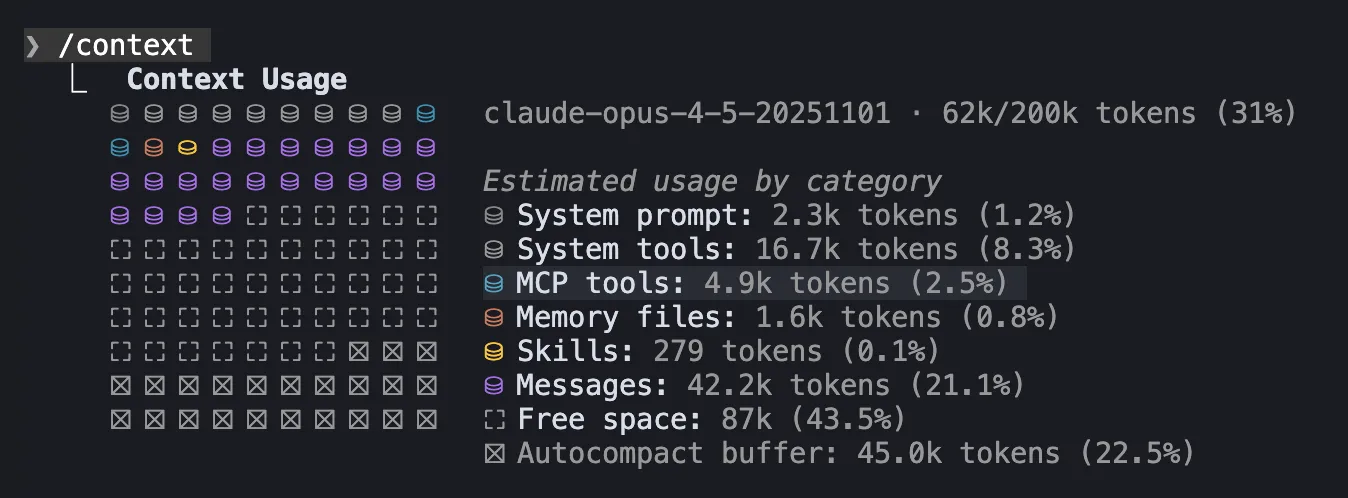
\includegraphics[width=0.62\linewidth]{figures/context-usage.png}\end{center}
\vskip4mm
\begin{tcbitemize}[cardsS, raster columns=2]
  \carditemplain{What it is}{Everything the model can see at once: your messages, every file it
    read, every command's output. The window has a fixed size.}
  \carditemplain{Why it matters}{As it fills, the earliest instructions get crowded out. A long
    thread does not get wiser. It gets vaguer.}
\end{tcbitemize}
\vfill
\end{frame}
\tanote{Show them this on your own screen if you can: type /context in Codex or Claude Code and it
draws the same picture. Two things to point at. The window holds the whole conversation, not just
your last message, so every file it opened and every command it ran is still in there taking up
room. And it is finite: when it runs out the tool starts dropping the oldest part, which is usually
your original instructions. That is the reason behind the rule in standard 3 - after twice round on
the same failure, start a new thread rather than arguing in the old one. It is also why a Ralph
loop hands each run a fresh agent. If someone asks how big: a few hundred thousand words, and
growing every year, but the habit matters more than the number.}

% ── 10b · context rot
% The U is the published shape, not decoration: performance is high at the ends of the window and
% sags in the middle, which is also the argument for what compaction throws away.
\hue{NovaPurple}
\begin{frame}{Context rot.}
\framesubtitle{What is an agent? · why a long thread goes stale}
\vspace*{\fill}
\noindent%
\begin{tikzpicture}[x=1mm, y=1mm]
  \useasboundingbox (0,-7) rectangle (134,21);
  \node[gp eyebrow=NovaMuted] at (0,17.6) {\lsp[13]{HOW WELL IT USES WHAT IS THERE}};
  \draw[NovaLine, line width=0.9pt] (0,0) -- (134,0);
  \draw[NovaAccent, line width=1.9pt] (2,14.5) .. controls (38,1.4) and (96,1.4) .. (132,14.5);
  \node[gg dot=NovaAccent] at (2,14.5) {};
  \node[gg dot=NovaAccent] at (132,14.5) {};
  \node[gg dot=NovaMuted]  at (67,4.7) {};
  \node[gp body, anchor=north west] at (0,-1.6) {the start of the thread};
  \node[gp body, anchor=north]      at (67,-1.6) {everything in the middle};
  \node[gp body, anchor=north east] at (134,-1.6) {what you just said};
\end{tikzpicture}%
\vskip3mm
\begin{tcbitemize}[cardsS, raster columns=3]
  \carditemplain{It is measured}{Eighteen models tested. Every one got worse as the input grew,
    well short of the limit.}
  \carditemplain{Lost in the middle}{It uses the start and the end. The middle goes soft — and
    that is where your bug is.}
  \carditemplain{So: compact}{Keep a summary and what just happened, drop the rest. A
    million-word window is not a memory.}
\end{tcbitemize}
\vskip2mm
{\tiny\color{NovaMuted}Liu, N. F.\ et al.\ (2024). \emph{Lost in the Middle: How Language Models
Use Long Contexts.} TACL 12 · arxiv.org/abs/2307.03172 · Chroma (2025), \emph{Context Rot}}
\vfill
\end{frame}
\tanote{Windows went 8k, 32k, 128k, a million. The number on the box grew a hundredfold; how well
the model uses the middle of it did not. Liu et al.\ measured the U shape in 2024 and it has held
for every model family since — Chroma re-ran it across eighteen models in 2025 and every one of
them degraded with input length, including well short of the limit. Two things follow, and both
are already rules in this deck. Start a new thread rather than arguing in a long one. And
compaction is not the tool being lazy: it is deliberately discarding the part the model was using
worst, and keeping the two parts it uses best. If you have the screen, run /context and then
/compact so they see the bar drop.}

% ── 10 · the long run-up
\hue{NovaPurple}
\begin{frame}{The long run-up.}
\framesubtitle{How we got here}
\vskip3mm
\noindent%
\begin{tikzpicture}
  \useasboundingbox (0,-21mm) rectangle (0.994\linewidth,12mm);
  \tlband{0.01}{0.17}{NovaMuted}{the idea}
  \tlband{0.21}{0.37}{NovaYellow}{the winter}
  \tlband{0.41}{0.77}{NovaAccent}{the answers}
  \tlband{0.81}{0.98}{NovaPurple}{the shape}
  \draw[tl axis] (0,0) -- (\linewidth,0);
  \tlstop{0.10}{NovaMuted}{1958}{Perceptron}{learns from examples}{17mm}
  \tlstop{0.29}{NovaYellow}{1969}{\emph{Perceptrons}}{one layer cannot do XOR}{20mm}
  \tlstop{0.49}{NovaAccent}{1986}{Backpropagation}{many layers, trainable at last}{20mm}
  \tlstop{0.69}{NovaAccent}{1997}{LSTM}{memory across a sequence}{20mm}
  \tlstop{0.89}{NovaPurple}{2017}{Transformer}{attention, and it scales}{20mm}
\end{tikzpicture}%
\vskip8mm
\vskip4mm
\muted{The ideas were all there. \textbf{Something else was missing.}}
\vfill
\end{frame}
\tanote{Ninety seconds, left to right. The dates are on the slide; the names and the story are
here. 1958,
Rosenblatt's perceptron: a machine that adjusts its own weights from examples instead of being
programmed rule by rule. That is still the whole idea. 1969, Minsky and Papert's book
\emph{Perceptrons}: one layer can only separate what a straight line separates, so it cannot learn XOR, about as simple as a function gets. Funding collapsed; the first AI winter. Careful with the
attribution: Minsky did not invent multi-layer networks. Everyone knew more layers would fix XOR;
nobody could train them. His critique is what made that the open problem. 1986, Rumelhart, Hinton
and Williams in Nature: backpropagation sends the error back through every layer, so many layers
finally become trainable. The answer to 1969, seventeen years late. 1997, Hochreiter and
Schmidhuber: LSTM carries memory across a sequence. 2017, Vaswani et al.: the Transformer drops
recurrence for attention and trains in parallel. Every model two slides from now is one of these.
If it comes up: Hinton shared the 2024 Nobel Prize in Physics with John Hopfield for this line of
work.}

% ── 11 · what actually changed
\hue{NovaPurple}
\begin{frame}{Why it happened now.}
\framesubtitle{How we got here}
\vspace*{\fill}
\begin{tcbitemize}[cardsS, raster columns=2]
  \carditem{Compute}{Arithmetic got cheap}{In 2007 graphics cards became programmable. In 2012
    a network trained on two of them won the image contest.}
  \carditem{Data}{The web became a corpus}{Since 2007 a non-profit has crawled the public web and
    given it away. Billions of pages, free.}
\end{tcbitemize}
\vskip6mm
\muted{Neural nets are not new. \textbf{Cheap parallel arithmetic and a scraped web are.}}
\vskip3mm
{\tiny\color{NovaMuted}NVIDIA CUDA (2007) · Krizhevsky, Sutskever \& Hinton, AlexNet (2012) ·
Common Crawl (founded 2007, public crawls from 2011)}
\vfill
\end{frame}
\tanote{This is the payoff of the previous slide. The ideas sat there for
decades because the two things they needed had not arrived. \textbf{Compute} — NVIDIA's CUDA (2007)
let ordinary programmers run their own maths on a graphics card, which is thousands of tiny
arithmetic units built for game pixels, which turned out to be what a neural network needs.
In 2012 AlexNet — Krizhevsky, Sutskever and Hinton — trained on two consumer GPUs and won the
ImageNet competition with roughly half the error of the runner-up; that is the moment it became
obvious to everyone. \textbf{Data} — Common Crawl, a non-profit founded in 2007 publishing
full-scale crawls from 2011: the web itself, free, as a training corpus. Neither one is an idea
about intelligence. If someone asks why this happened now and not in 1990, that is the answer.}

% ── 12 · chronology
\hue{NovaPurple}
\begin{frame}{2018 onwards.}
\framesubtitle{How we got here}
\vskip3mm
\noindent%
\begin{tikzpicture}
  \useasboundingbox (0,-30mm) rectangle (\linewidth,11mm);
  \tlband{0.01}{0.23}{NovaMuted}{completing}
  \tlband{0.27}{0.61}{NovaYellow}{conversing}
  \tlband{0.65}{0.87}{NovaAccent}{acting}
  \tlband{0.88}{0.98}{NovaPurple}{persisting}
  \draw[tl axis] (0,0) -- (\linewidth,0);
  \tlstop{0.06}{NovaMuted}{2018}{GPT-1}{continues text}{19mm}
  \tlstop[11mm]{0.19}{NovaMuted}{2019}{GPT-2}{coherent paragraphs}{19mm}
  \tlstop{0.32}{NovaYellow}{2020}{GPT-3, Codex}{learns from the prompt}{19mm}
  \tlstop[11mm]{0.45}{NovaYellow}{2022}{ChatGPT}{follows instructions}{19mm}
  \tlstop{0.58}{NovaAccent}{2023}{GPT-4}{tool calling}{19mm}
  \tlstop[11mm]{0.71}{NovaAccent}{2024}{Reasoning}{thinks before it acts}{19mm}
  \tlstop{0.84}{NovaAccent}{2025}{Harnesses}{builds in your repo}{19mm}
  \tlstop[11mm]{0.93}{NovaPurple}{2026}{Long-running}{works while you are away}{18mm}
\end{tikzpicture}%
\vskip5mm
\vskip1mm
\muted{The job changed twice: when it learned to take \textbf{instructions}, and when it got
\textbf{tools and a loop}.}
\vfill
\end{frame}
\tanote{Two minutes, one sweep left to right. Sixty years fitted onto the last two slides; these
eight get their own because this is where the job changed, not just the size. Say the four band names as you go (completing, conversing, acting, persisting). That is the shape to remember, not the model names. If asked for
an example of reasoning: an older model asked why the balances were wrong guesses a plausible edit;
a reasoning model works the arithmetic out and lands on the actual line. Dates are approximate
release months on purpose.}

% ═════════════════════════════════════════════ ACT 2 · three standards
\sectionslide[NovaAccent]{3}{The core of the class}{Three standards.}%
{A rulebook it reads. A judge it cannot argue with. A loop that knows when to stop.}

% ── 9 · standard 1
\hue{NovaYellow}
\begin{frame}{\codetitle{AGENTS.md}}
\framesubtitle{Standard 1 · The rulebook}
\vspace*{\fill}
\begin{tcbitemize}[cardsS]
  \carditem{What it is}{A README for agents.}{Every session starts by reading it.}
  \carditem{What goes in}{What it cannot guess.}{Commands. Boundaries. How to report back.}
  \carditem{What stays out}{What it can read.}{Your code, explained. Every extra line hides a real
    one.}
\end{tcbitemize}
\vskip6mm
\muted{It lives in git. When the agent misbehaves, the fix is usually a line here.}
\vfill
\end{frame}
\tanote{Ask Codex on stage: "What does AGENTS.md tell you to do?" It recites the file. That is the
proof it reads it. The test for every line: would removing it cause a mistake? If not, cut it.
Mention the 32 KB cap only if asked; the real cap is attention.}

% ── 10 · the three rules
\hue{NovaYellow}
\begin{frame}{Three rules.}
\framesubtitle{Standard 1 · Live · 4 min}
\vspace*{\fill}
\begin{tcbitemize}[cardsS]
  \carditem{Boundary}{One branch per spec.}{Never straight to \code{main}.}
  \carditem{Evidence}{Show me the test output.}{The output itself, not a summary of it.}
  \carditem{Off-limits}{Never touch the tests.}{If one looks wrong, say so and stop.}
\end{tcbitemize}
\vskip6mm
\muted{Exact wording on the Week 4 page. Add them, read the diff, commit, push.}
\vfill
\end{frame}
\tanote{Do it on stage: ask Codex to add the three rules under "How to answer" in AGENTS.md, read
the diff aloud, accept, commit in GitHub Desktop. The third already existed in spirit; now it is explicit, and the student enforces it. Codex only reads AGENTS.md at the start of a thread, so say
"new thread" now.}

% ── 11 · standard 2
\hue{NovaAccent}
\begin{frame}{The judge.}
\framesubtitle{Standard 2 · 5 min}
\vspace*{\fill}
\begin{tcbitemize}[cardsS, raster columns=2]
  \carditem{The problem}{So give it a check.}{Failing tests are the to-do list.
    Green is the finish line.}
  \carditem{The rule}{Editing a test is cheating.}{It is not finishing.}
  \carditem{Evidence}{Show me the output.}{Anyone can type ``all tests pass''.}
    \carditem{After green}{Read the diff. Click the app.}{App wrong, tests green? You found a
    missing test.}
\end{tcbitemize}
\vskip5mm
\muted{Decide what \emph{done} means before you start.}
\vfill
\end{frame}
\tanote{Run the red tests on stage (command on the Week 4 page) and open the test file next to the
spec: one test per checklist line. "Green is not done" is the card that pays off today: feature 2's
form field is not tested at all, so only clicking the app catches a missing one.}

% ── 12 · standard 3
\hue{NovaAccent}
\begin{frame}{The loop.}
\framesubtitle{Standard 3 · 5 min}
\diagram[1.0\linewidth]{figures/loop.pdf}
\vskip1mm
\begin{tcbitemize}[cardsS]
  \carditemplain{One task per loop}{One bug, or one spec.}
  \carditemplain{Let it loop}{It reads its own failures. You read the result.}
  \carditemplain{Know when to stop}{Green. Or twice round on the same failure, and then a new thread.}
\end{tcbitemize}
\vfill
\end{frame}
\tanote{The three parts are the whole lesson: a rulebook, a judge, a loop. Everything else in
agentic coding is a variation. Today the loop runs inside one Codex turn and you watch; the same
idea one level up is a script that re-feeds the prompt until the judge passes. Part II, Block 3.}

% ── 13 · the four parts of an ask
\hue{NovaAccent}
\begin{frame}{The shape of an ask.}
\framesubtitle{Standard 3}
\vspace*{\fill}
\begin{tcbitemize}[cardsS, raster columns=4]
  \carditem{1}{The task}{One thing. Name the spec.}
  \carditem{2}{The boundary}{This branch. Never the tests.}
  \carditem{3}{The judge}{Run the tests until they pass.}
  \carditem{4}{The evidence}{The output, and every file touched.}
\end{tcbitemize}
\vskip7mm
\muted{Written out in full on the Week 4 page. Copy it; change two names.}
\vfill
\end{frame}
\tanote{Four parts, in every loop prompt they will ever write. Make them name the four back to you
before you paste it. New thread before pasting: the AGENTS.md rules from five minutes ago are only
read at the start of a thread.}

% ── 14 · Ralph: the loop with nobody watching
\hue{NovaAccent}
\begin{frame}{Ralph.}
\framesubtitle{Standard 3 · nobody watching}
\vspace*{\fill}
\begin{center}\roundedpic[0.44\linewidth]{figures/ralph.jpg}\end{center}
\vskip3mm
\begin{tcbitemize}[cardsS, raster columns=2]
  \carditemplain{What it is}{The same prompt, handed to a fresh agent again and again, until the
    judge says green.}
  \carditemplain{Why a crowd}{Every run is a new one, and none remembers the last. What they need
    to know has to be written down.}
\end{tcbitemize}
\vfill
\end{frame}
\tanote{Thirty seconds. You are not demoing this today. Named after Ralph Wiggum: cheerfully,
relentlessly wrong, and he gets there anyway. The picture is the technical point, not the joke —
there is no single agent getting better at the task. There is a queue of identical beginners, each
starting from nothing. Ask the room what that implies, and let someone say it: the files are the
only memory.}

% ── 15 · Ralph, in full: where it comes from and what holds it
\hue{NovaAccent}
\begin{frame}{Nobody is watching.}
\framesubtitle{Standard 3 · where Ralph comes from}
\vspace*{\fill}
\begin{center}\codeline{while :; do cat PROMPT.md | claude-code ; done}\end{center}
\vskip2mm
\begin{center}\muted{Published in 2025. That is the entire technique.}\end{center}
\vskip6mm
\begin{tcbitemize}[cardsS, raster columns=3]
  \carditemplain{The prompt}{One file, read again from scratch every time. It is the only
    instruction anyone gives.}
  \carditemplain{The repo}{Nothing survives a run except what was written to disk. The rulebook and
    the tests are the memory.}
  \carditemplain{The catch}{Nobody reads anything until it stops. A weak judge buys you hours of
    confident wrong.}
\end{tcbitemize}
\vskip2mm
% \code{} here would set a \small chip inside a \tiny line and tower over it
{\tiny\color{NovaMuted}Huntley, G. (2025). \emph{Ralph Wiggum as a ``software engineer''} ·
ghuntley.com/ralph · an official Claude Code plugin since December 2025}
\vfill
\end{frame}
\tanote{This is the slide that closes the act, so land it: rulebook, judge, loop are not three
tips. They are the three things that make an unattended agent safe to run at all. Huntley's own
line for why it works is "the technique is deterministically bad in an undeterministic world" —
bounded, repeatable failure plus a check that cannot lie. Worth the credibility beat: Anthropic
shipped it as an official Claude Code plugin in December 2025, and Boris Cherny, who built Claude
Code, has said he reaches for it on long-running tasks. Nobody should run this today. They should
recognise that the three standards are what make it possible.}

% ── 16 · the loop, shipped as a feature
% The visual rhyme with the slide before is the argument: same chip, same place on the page,
% one year apart. The loop got easier to run; the judge did not get easier to write.
\hue{NovaAccent}
\begin{frame}{\codetitle{/goal}}
\framesubtitle{Standard 3 · the loop, one year later}
\vspace*{\fill}
\begin{center}\codeline{/goal every test in tests/ passes, and nothing in tests/ changed}\end{center}
\vskip2mm
\begin{center}\muted{2026. The shell loop is now one sentence, in the tool.}\end{center}
\vskip6mm
\begin{tcbitemize}[cardsS, raster columns=3]
  \carditemplain{Who decides}{After each turn a \emph{second}, smaller model reads the
    conversation and rules: not yet, done, or impossible. Not the one doing the work.}
  \carditemplain{What it can see}{It cannot run your tests. It only reads what the agent put on
    screen. So the finish line has to be something the agent can show you.}
  \carditemplain{Still yours}{The tool runs the loop now. Nobody has automated deciding what
    \emph{done} means.}
\end{tcbitemize}
\vskip2mm
{\tiny\color{NovaMuted}Claude Code, \emph{Keep Claude working toward a goal} ·
code.claude.com/docs/en/goal · Codex ships the same command, behind \emph{features: goals}}
\vfill
\end{frame}
\tanote{This is the payoff of the whole act, so do not rush it. A year ago Ralph was a bash loop
you wrote yourself. Today both Claude Code and Codex ship it: /goal takes a finish line in plain
words and keeps taking turns until a separate evaluator model agrees it holds. Underneath it is
literally a Stop hook, which is what the ralph-wiggum plugin was. Two things to land. First: the
evaluator does not run anything — it only reads the transcript, which is exactly why "paste the
final test output" is in their loop prompt. Evidence is not politeness, it is the only thing the
judge can see. Second: everything the tool automated was the easy half. Nothing here writes the
rulebook or decides what done means. That is the job, and it is theirs. Students on Codex can turn
it on today; tell them it is in the handout, and that they should not use it until they have a
test that fails first.}

% ═════════════════════════════════════════════ ACT 3 · git, as one story
\sectionslide[NovaBlue]{git}{How a team stays sane}{One change, start to finish.}%
{\code{main} is the version everyone trusts. Here is how a change gets into it.}
\tanote{Five minutes for the whole story, about fifty seconds a slide. Four of the six are the
previous picture plus one move, so do not narrate them twice — point at what is new and go on.
They met repo, commit, branch and push last week as words; this is the same words as a single
narrative, in the shape they will actually see in GitHub Desktop. Frame it the way they already
think: a draft, checkpoints, a review, a sign-off.}

% ── git 1 · main
\hue{NovaBlue}
\begin{frame}{\codetitle{main}}
\framesubtitle{Git · 1 of 6}
\vspace*{\fill}
\gitgraph{1}
\vskip6mm
\muted{One version, one history, one truth. No folder full of
\emph{model\_v3\_FINAL\_jm}.}
\vfill
\end{frame}

% ── git 2 · branch
\hue{NovaBlue}
\begin{frame}{A branch.}
\framesubtitle{Git · 2 of 6}
\vspace*{\fill}
\gitgraph{2}
\vskip6mm
\muted{A \textbf{branch} is your own copy to work in, named after the job. Everyone else carries on
from \code{main}, undisturbed.}
\vfill
\end{frame}

% ── git 3 · commit
\hue{NovaBlue}
\begin{frame}{A commit.}
\framesubtitle{Git · 3 of 6}
\vspace*{\fill}
\gitgraph{3}
\vskip6mm
\muted{A \textbf{commit} is a checkpoint with a note saying what changed. Small ones. You can go
back to any of them.}
\vfill
\end{frame}

% ── git 4 · main has not moved
\hue{NovaBlue}
\begin{frame}{Working on a branch.}
\framesubtitle{Git · 4 of 6}
\vspace*{\fill}
\gitgraph{4}
\vskip6mm
\muted{Three commits in and half of it broken. Everyone else's copy is untouched.}
\vfill
\end{frame}

% ── git 5 · local and remote
% Two boxes, one history, two arrows. The chains sit at the same height in both cards on
% purpose: the point of the slide is that it is the same history, kept in two places.
\hue{NovaBlue}
\begin{frame}{Local, and remote.}
\framesubtitle{Git · 5 of 6}
\vspace*{\fill}
\noindent%
\begin{tikzpicture}[x=1mm, y=1mm]
  \useasboundingbox (0,-41) rectangle (134,5);
  % ── your laptop
  \node[gp eyebrow=NovaMuted] at (0,1.4) {\lsp[13]{YOUR LAPTOP · LOCAL}};
  \path[gp card=NovaCard] (0,-1) rectangle (62,-38.5);
  \node[gp head] at (31,-4.4) {the folder you edit};
  \node[gp file, anchor=west] (fa) at (12,-12.5) {app.py};
  \node[gp file, anchor=west] (fb) at ($(fa.east)+(2.4mm,0)$) {tests/};
  \node[gp file, anchor=west] (fc) at ($(fb.east)+(2.4mm,0)$) {AGENTS.md};
  \draw[gp move=NovaMuted] (31,-17) -- (31,-23);
  \node[gp movelabel=NovaFg, anchor=west] at (33,-20) {commit};
  \gpchain{19}{43}{-28}{NovaTeal}
  \node[gp body] at (31,-31.4) {your history};
  % ── github: the same chain, at the same height, with the rest of the team above it
  \node[gp eyebrow=NovaBlue] at (86,1.4) {\lsp[13]{GITHUB · THE REMOTE}};
  \path[gp card=NovaBlueBg] (86,-1) rectangle (134,-38.5);
  \node[gp head] at (110,-4.4) {one copy, shared};
  \gpchain{98}{122}{-14}{NovaBlue!32}
  \gpchain{98}{122}{-21}{NovaBlue!32}
  \gpchain{98}{122}{-28}{NovaTeal}
  \node[gp body] at (110,-31.4) {yours, and everyone else's};
  % ── the two moves
  \draw[gp move=NovaMuted] (64.5,-21) -- (83.5,-21);
  \node[gp movelabel=NovaFg, anchor=south] at (74,-20.1) {push};
  \node[gp body] at (74,-22.1) {your branch, up};
  \draw[gp move=NovaMuted] (83.5,-33) -- (64.5,-33);
  \node[gp movelabel=NovaFg, anchor=south] at (74,-32.1) {pull};
  \node[gp body] at (74,-34.1) {their work, down};
\end{tikzpicture}%
\vskip4mm
\muted{\textbf{Push} sends your branch to the copy everyone shares, where a \textbf{pull request}
asks someone to read the diff first. Today that someone is you, reviewing the agent.}
\vfill
\end{frame}
\tanote{The only slide in the act that leaves the graph, and the one that fixes the vocabulary:
\emph{local} is the copy on your laptop, \emph{remote} is the copy on GitHub. Point at the two
chains drawn at the same height and say it plainly — it is one history, kept in two places, and
push and pull are the only things that move between them. The grey chains above yours are the rest
of the team. If someone asks where "add"/"staging" went: GitHub Desktop turned it into the
checkboxes next to each changed file, so they have already used it without the name.}

% ── git 6 · merge
\hue{NovaBlue}
\begin{frame}{Merge.}
\framesubtitle{Git · 6 of 6}
\vspace*{\fill}
\gitgraph{5}
\vskip6mm
\muted{\textbf{Merge} is the sign-off. \code{main} now has your work, and the next person starts
from there.}
\vfill
\end{frame}
\tanote{Land the cycle: they are back at slide one, with a bigger main. That is the
habit. Two rules fall out of the story rather than being announced: name the branch after the job
(slide 2), and keep commits small enough to explain (slide 3). If someone asks what happens to the
branch: it is finished, GitHub offers to delete it, say yes.}

% ═════════════════════════════════════════════ ACT 4 · do it
\hue{NovaTeal}
\begin{frame}{Feature 2, live.}
\framesubtitle{Live · 10 min}
\vspace*{\fill}
\begin{steps}
  \item \textbf{Branch.} Named after the spec.
  \item \textbf{Red first.} See what is missing before anything is written.
  \item \textbf{New thread. Paste the ask.} Then sit on your hands.
  \item \textbf{Watch it loop.}
  \item \textbf{Green — now don't trust it.} Read the diff. Click the app.
  \item \textbf{Commit, push, pull request, merge.}
\end{steps}
\vfill
\end{frame}
\tanote{Let it loop for real; 2-4 rounds is normal. Narrate it as tool calls. Commands and file
names are on the Week 4 page if you want them on screen. The two things it commonly misses on this
feature: it forgets to refresh the data files from the seed (tests stay green while the app crashes
on load) and it never adds the form field (nothing tests that screen). Both are the "green is not
done" lesson. Show them, do not fix them silently. If it edits a test: stop, discard, point at the
rule, re-prompt.}

% ── 19 · your turn
\hue{NovaTeal}
\begin{frame}{One bug, then feature 2.}
\framesubtitle{Your turn · 30 min}
\vspace*{\fill}
\begin{tcbitemize}[cardsS, raster columns=2]
  \carditem{SplitIt}{Bug 2, then feature 2}{Removing a member crashes the page. Then expense
    categories.}
  \carditem{Tiny CRM}{Bug 3, then feature 2}{``Won this month'' is always zero. Then conversion by
    source.}
\end{tcbitemize}
\vskip7mm
\muted{Files, test names and the ask: Week 4 page.}
\vfill
\end{frame}
\tanote{Roam for two things: did they ask for the test output, and did they read the diff before
accepting. Never answer a failing test. Ask "what does the last line say?". SplitIt bug 002: the test
demands a helper that also removes the member's expenses; the assertion message says so. Tiny CRM
bug 003 has a twist: stamping the close date is not enough. The month counter gives up on the whole
list when any won lead has no date, and the seed has five; the fix is to skip them, not return zero.
Anyone still on feature 1 does that first; feature 2 becomes homework.}

% ── 20 · when it goes wrong
\hue{NovaAccent}
\begin{frame}{When it goes wrong.}
\framesubtitle{Your turn}
\vspace*{\fill}
\begin{steps}
  \item \textbf{It edited a test.} Discard. Say the rule. Run again.
  \item \textbf{``Done'' — tests red.} Ask for the output.
  \item \textbf{Same failure, three times.} Stop. Read it yourself. New thread.
  \item \textbf{It fixed three other things.} Discard. One task per loop.
  \item \textbf{Green, app wrong.} Write down what the judge missed.
\end{steps}
\vskip6mm
\muted{Every line here is a candidate rule for your \code{AGENTS.md}.}
\vfill
\end{frame}

% ── 21 · retro
\hue{NovaYellow}
\begin{frame}{Write one rule.}
\framesubtitle{Retro · 6 min}
\vspace*{\fill}
\begin{itemize}
  \item The worst thing it did today — one sentence.
  \item Turn it into a rule you could check.
  \item Commit it to \code{AGENTS.md}, with the reason.
\end{itemize}
\vskip7mm
\muted{A rulebook grows one line at a time, from things that went wrong.}
\vfill
\end{frame}
\tanote{Collect the rules on the board; the good ones become the course's AGENTS.md for Block 2.
Expect: "refresh the data after changing the seed files", "don't edit live data by hand", "show me
the diff before committing". Reject vague ones ("be careful"). Ask "how would you know it followed this?".}

% ── 22 · wrap
\hue{NovaTeal}
\begin{frame}{Before next week.}
\framesubtitle{Class 4 · wrap}
\vspace*{\fill}
\begin{itemize}
  \item Feature 2: green, merged, pushed.
  \item One new rule in \code{AGENTS.md}.
  \item Push before you close the laptop.
\end{itemize}
\vskip9mm
{\displayfont\Large\bfseries\color{NovaFg}Rulebook \textcolor{NovaMuted}{·} judge
\textcolor{NovaMuted}{·} loop.}
\vfill
\end{frame}
\tanote{Nothing to hand in. Next week's check-in: feature 2 merged, and a commit on AGENTS.md.
Part II of the standards — walking away: scripted loops, goals, a second agent reviewing — comes
with the team project in Block 3.}

\end{document}
